\documentclass[]{article}

\usepackage{listings}
\usepackage{appendix}
\usepackage{hyperref}
\usepackage{graphicx}

% This is only possible with lualatex
\usepackage{fontspec}
\setmainfont[Ligatures=TeX]{Raleway}

\def\code#1{\texttt{#1}}

% New macro so we can easily reference source files
\newcommand{\gitlab}[1]{\footnote{See \href{https://gitlab.com/YottaDB/DBMS/YDBOcto/blob/master/#1}{#1}}}

%opening
\title{Creating a SQL Engine for NoSQL Databases}
\author{Charles Hathaway, Jon Badiali, Narayanan Iyer, KS Bhaskar}


\begin{document}

\maketitle

\tableofcontents

\begin{abstract}
	
	There is plenty of research talking about specific details of implementing a SQL engine and query optimizer, but very little direction given for the more mundane task of actually creating one.
	Knowledge of the field of programming languages and database systems is required to even begin the task, but each of those fields is so large that gaining a breadth of understanding can take years.
	In this paper, we explore the creation of Octo - a SQL engine designed to provide access to data that already exists in YottaDB datastores, such as the wealth of information generated by users of the VistA EHR system.

\end{abstract}


\section{Introduction}

Octo maps data stored in M globals to a relational schema overlay using an augmented SQL DDL language.
The user is responsible for generating this DDL, and informing Octo about how to fetch specific columns and iterate through data in a table.
With these pieces of information, Octo can generate execution plans for a given SQL query, including JOINs, which return the data the user is looking for.
Octo uses a 3-phase architecture, consisting of parsing, logical plan generation and optimization, and physical plan generation and emission.
Each of these phases is explored in detail in the following sections.

Throughout this document, we make use of examples referencing a sample schema.
This schema is intentionally very simple, allowing us to keep the sample queries and generated plans small and manageable.
Please see listing \ref{fig:intro_names_schema} for the source DDL, and listing \ref{fig:into_names_data} for the data we use when executing these queries.

Note that the GLOBAL keyword in listing \ref{fig:intro_names_schema} is explained in section \ref{sec:parsing}.
For now, just know that it is glue connecting the underlying M database to the relational schema.


\section{Background Information}

% We should write something describing M globals here

\subsection{Mapping Non-relational Schemas to Relations} \label{sec:background_mapping}

\section{Parsing} \label{sec:parsing}

The first step in handling a SQL query is to parse it.
SQL has a standard, formalized by the American National Standards Institute, with revisions every few years.
One of the most common target standard versions is SQL-92 (the 1992 standard), as this includes most of what people expect from SQL, but is not too complicated.
Octo aims to be compatible with this version, using SQL: The Standard Handbook \cite{cannan1993sql} as a reference manual, with the primary source for the grammar described at \url{https://github.com/ronsavage/SQL/blob/master/sql-92.bnf}\cite{ronsavage2003sql}.
However, this grammar includes some structures which are not friendly towards the parsing generator selected, so the grammar was refactored in places to prevent parsing errors.
For the current grammar, look at \gitlab{src/parser/parser.y}.

The initial time frame for getting a working prototype did not allow for the development of a recursive descent parser, and performance concerns did not allow the use of newer parse-tree parsers (such as ANTLR \cite{parr2013definitive} \footnote{There is some contention about ANTLR vs Bison performance, and a judgement call was made based on small performance tests and community discussion}, and overall generalized LR parsers \cite{lang1974deterministic}).
This, along with other constraints imposed by the development environment, forced Octo into using a C toolchain, which requires using tools such as YACC/Bison and Flex over more modern solutions.

\subsection{Recap: LALR(1) Parsing Algorithm}

The topic of parsing programming languages and deriving semantic meaning from the parsed tree is a complex one, which often has several graduate level computer science classes devoted to it.
Although parsing a SQL grammar doesn't share the same type of complexity as a class on compiler design, there are definite overlaps, and a solid foundation in this area will help with understanding the first few phases of the Octo pipeline.
Readers are encouraged to read up on core programming language concepts in books such as Programming Language Pragmatics \cite{scott2000programming}.
However, for the purpose of clarity, we will give a brief explanation about the nature of Octo's parser here to help those hoping to gain insight from it.

As described in section \ref{sec:parsing}, Octo uses YACC/Bison to read in a grammar and produce a LALR(1) parsing table.
LALR(1) is a look-ahead left-right parser, with 1 token of look-ahead.
It is very similiar to more general LR algorithms, which is what we describe below.
The key difference is the disinction of states in the generated FSM.
To understand the algorithm, we need to know a few terms.

\begin{itemize}
	\item Token -- A 'keyword' from the grammar which is represented in Bison as an enum value. This is the output of the lexing phase. These are also known as terminating symbols.
	\item Rule -- Anything that is not a token in the grammar is a rule. A rule contains subrules, which can recurse or terminate in tokens. These are also known as non-terminating symbols.
	\item $FOLLOW$ set -- Given a state, this is the list of tokens which can follow from this state.
	\item $FIRST$ set -- The first token which may appear in the grammar.
\end{itemize}

\lstinputlisting[
caption={Sample calculator grammar},
label=fig:parser_sample_calc_grammar]
{figures/parser_calc.y}

Listing \ref{fig:parser_sample_calc_grammar} contains the sample grammar we will use for a concrete example of the algoritm.
The first thing in this listing is a list of tokens which represent terminating symbols.
For a real application, there would be a lexer (written, for example, flex) which parses an input stream and splits it into tokens for Bison to consume.
We define 5 tokens; PLUS, MINUS, MULT, DIV, and LITERAL.

Shortly after, we have the rules that we use to define the grammar.
To imagine how the parse table is constructed, we must first identify all possible states.
We begin by capturing the $FIRST$ set.
This is the set of tokens that are the first tokens we encounter in our stream.
If we trace through the grammar, we go $term \rightarrow factor \rightarrow LITERAL$, which yields a LITERAL token as a first token.
We must also go down all possible paths in the grammar, so in addition to matching the first terminal in the factor rule, we delve into the term rule and go $\rightarrow term \rightarrow LITERAL$.
Since this also yields a LITERAL token, our $FIRST$ set contains a single token: LITERAL.

This brings us to the first field in our parse table.
In this representation of the parse table, rows represent states, and columns represent tokens.

\begin{center}
	\begin{tabular}{| c | c | c |}
		\hline
		& LITERAL      & \\
		\hline
		state 0 & goto state 1 & \\
		\hline
	\end{tabular}
\end{center}

Next, we must calculate state 1's $FOLLOW$ set.
Conceptually, this is just any token that can follow a literal; an easy (but non-rigorous) method to find it is to look for anything which can follow a LITERAL.
For a more rigorous approach, look at programming language textbooks for a formal definition.

In factor, we see LITERAL can be followed by factor, or nothing (aka, the end of the input string, aka $\epsilon$).
Since we know factor can be a LITERAL, we must also include MULT and DIV.
Through the same reasoning, we can determine that term can become a LITERAL, and we must include PLUS and MINUS.
So our $FOLLOW$ set for state 0 is $\{MULT, DIV, PLUS, MINUS, \epsilon\}$.
We can add some states to our table for this.

\begin{center}
	\begin{tabular}{| c | c | c | c | c | c | c | c |}
		\hline
		& LITERAL      & MULT & DIV & PLUS & MINUS & $\epsilon$ \\
		\hline
		state 0 & goto 1 & & & & & \\
		state 1 &  & goto 2 & goto 2 & goto 3 & goto 3 & reduce \\
		\hline
	\end{tabular}
\end{center}

If we see the $\epsilon$ character, we know we are at the end of the input token stream, and can terminate the parse.
If we are in state 1 and see the $\epsilon$, it means we saw a single LITERAL by itself.
We can reduce (yield the first part of the parse; we no longer need to keep looking, a rule has been fully satisfied and can be removed from the stack).

Then we begin filling out for each remaining state.

\begin{center}
	\begin{tabular}{| c | c | c | c | c | c | c | c |}
		\hline
		& LITERAL      & MULT & DIV & PLUS & MINUS & $\epsilon$ \\
		\hline
		state 0 & goto 1 & & & & & \\
		state 1 &  & goto 2 & goto 2 & goto 3 & goto 3 & reduce \\
		state 2 & reduce & & & & & \\
		state 3 & reduce & goto 2 & goto 2 & goto 3 & goto 3 & \\
		\hline
	\end{tabular}
\end{center}

As we transition from state to state, we also 'shift' tokens off of the parse stream.
This effectively consumes the token, and advances to the next rule.

The last thing to note is that the LALR contributes to the general LR algorithm by merging states, which reduces code size and execution time.
The same rules apply for understanding shift/reduce and reduce/reduce errors.
See figure \ref{fig:parser_generated_graph} for the generated state diagram of the grammar given in listing \ref{fig:parser_sample_calc_grammar}.

\begin{figure}
	\begin{center}
		\makebox[\textwidth]{
			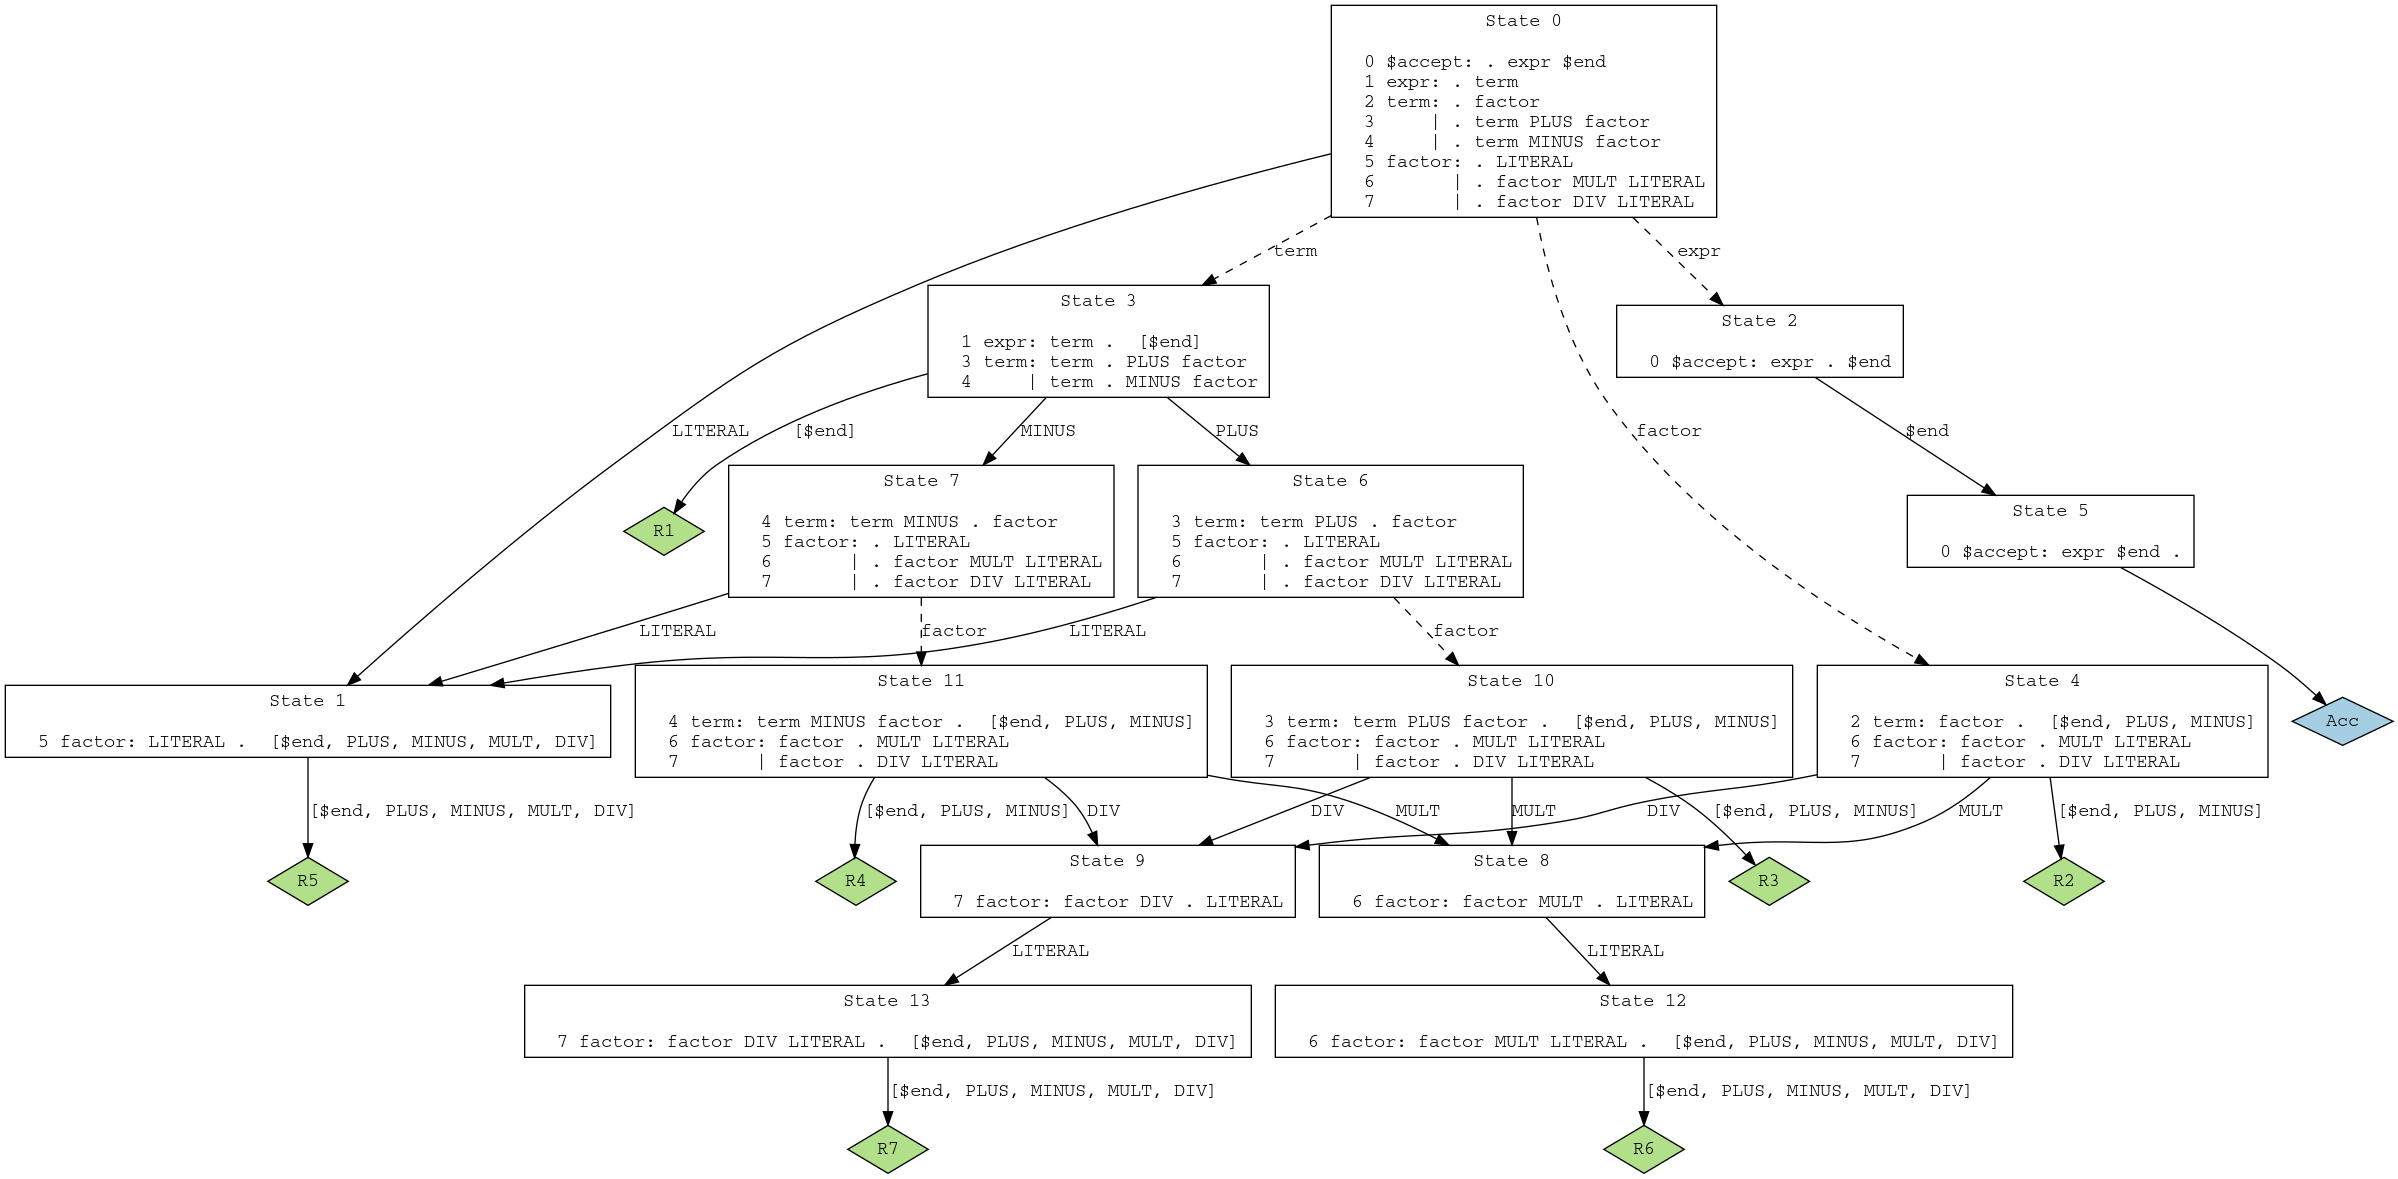
\includegraphics[width=.8\paperwidth]{figures/parsing_generated_graph.png}
		}
	\end{center}
	\label{fig:parser_generated_graph}
	\caption{Generated LALR state machine for sample grammar}
\end{figure}

%% TODO: charles isn't done here, and there are a few errors above

% prefix = lp_
\section{Logical Planning}

Logical planning is where a majority of the complexity of the SQL engine is located in this design; it includes things such as boolean expression expansion and reordering, converting JOIN's to a series of key iterations, transforming OUTER JOINs to a series of SET operations, and things of the like.

In Octo, logical planning first takes the data structures representing the parsed SQL query, and transforms it into a binary tree.
This binary tree is what we mean when we talk about the logical plan.
Later, optimizations are done on this tree which do things such as:

\begin{enumerate}
	\item Load keys from tables and insert them in a particular order to the 'keys' section of the logical plan
	\item Update keys to have specific advanced techniques, such as fixing them to a particular value if we know the boolean condition of the query requires the key to have that value
	\item Replace keys with cross-reference keys if we can perform an optimization on a column other than a key column
	\item Normalize boolean expressions to have no disjunctions, which would prevent other optimizations from taking place
\end{enumerate}

These items are explained in detail in section \ref{sec:lp_optimization}.

\subsection{Pre-optimization Logical Plans}

Before performing any optimizations, Octo converts the parsed SQL expression from the previous stage into a logical plan \gitlab{src/optimization\_transforms/generate\_logical\_plan.c}.
This logical plan is represented as a binary tree, where each element in the tree either has children. The type of children is dependent upon the type of element, and eventually terminates with a leaf node.
It is during this phase that we:

\begin{itemize}
	\item Expand certain expressions to more normalized expressions
	\begin{itemize}
		\item Specifically, much of this work is done in lp\_generate\_where \gitlab{src/optimization\_transforms/lp\_generate\_where.c}, and includes converting IN lists (i.e., \code{column\ IN\ ('1', '2', '3')}) into a series of disjunctive OR statements which we can later optimize
		\item If we detect a regex operator here with a second argument that starts with a \code{\^}, ends with a \code{\$}, and has no other regex characters, we convert it to a EQUALS statement
		\item Several \code{Sql*} structures (such as \code{SqlValue}) are encapsulated in \code{LP\_} structures (such as \code{LP\_VALUE})
	\end{itemize}
	\item Replace references to derived tables with references to their output keys
	\begin{itemize}
		\item Calls in \code{generate\_logical\_plan} to \code{replace\_table\_references}\gitlab{src/replace\_table\_references.c} are the primary means by which this happens, but calls to \\ \code{lp\_replace\_derived\_table\_references}\gitlab{src/optimization\_transforms/lp\_replace\_derived\_table\_references.c} can also replace code in some cases
	\end{itemize}
	\item Move JOIN conditions onto the WHERE condition
	\begin{itemize}
		\item This is done in \code{generate\_logical\_plan}, and relies on helper functions such as \code{lp\_join\_where}\gitlab{src/optimization\_transforms/lp\_join\_where.c} to keep the code manageable
	\end{itemize}
	\item Recurse into subplans to perform logical plan generation and optimization
	\begin{itemize}
		\item In cases where we encounter a subplan, either through walking trees in \code{lp\_generate\_where} or through SET operations (in which case we go through \code{lp\_generate\_set\_logical\_plan}\gitlab{src/optimization\_transforms/lp\_generate\_set\_logical\_plan.c})
	\end{itemize}
\end{itemize}

Consider figure \ref{fig:lp_before_optimizations} for an example of a logical plan.

\begin{figure}
	\lstinputlisting{figures/lp_before_optimization.yml}
	\caption{Logical plan without any optimizations performed. Source query: \texttt{select * from names;}}
	\label{fig:lp_before_optimizations}
\end{figure}

In this example, we can see the core structure of the base SELECT statement after it gets transformed.
Walking down this tree in a depth-first fashion, we can see:

\begin{itemize}
	\item At the top-level is a \code{LP\_INSERT}; this is meant to denote the semantic understanding that we are inserting data from the next \code{LP\_PROJECT} into a \code{LP\_OUTPUT}.
	\item \code{LP\_PROJECT}, which represents a relational projection of data. In addition to the column selection list, we also store data about the criteria for selection and the source of the selections.
	\item \code{LP\_COLUMN\_LIST} is a top-level item which will have a value/expression node on the left, and another \code{LP\_COLUMN\_LIST} or a NULL value on the right.
	\item \code{LP\_WHERE} marks the beginning of an expression. Originally used only in the WHERE clause of the SQL expression, as Octo evolved, it found use in many other places, including to represent expressions in the projection. Generally, the right-hand expression of a \code{LP\_WHERE} is allowed to be NULL, however, in some places it is overloaded to store additional information specific to the context; this is one such place, where we store the \code{LP\_COLUMN\_LIST\_ALIAS} description in the right node, and the expression in the left node.
	\item \code{LP\_COLUMN\_ALIAS} is one of many nodes that can be part of an expression; specifically, \code{LP\_COLUMN\_ALIAS} refers to a column in one of the joined table, and is a leaf node that includes information such as table and column names.
	\item \code{LP\_COLUMN\_LIST\_ALIAS} stores information about how this column list should be referred to later in the plan, including in parent/children queries, within the WHERE/ORDER BY clauses, etc. It is a leaf node that contains an alias (column name) and the type of the data item.
	\item \code{LP\_SELECT} is a parent node which represents a 'select' criteria, including source tables and conditions of the selection.
	\item \code{LP\_TABLE\_JOIN} has a table in the left node, and either NULL or a \code{LP\_TABLE\_JOIN} in the right join. Internally, this does include information about the conditions of the join, but they are not currently rendered in the logical plan.
	\item \code{LP\_CRITERIA} contains information about the limitations of our table select, including boolean conditions. After being optimized, the left node will contain a list of keys which are used in physical selection of data from the database. The right node stores the options of the select.
	\item \code{LP\_KEYS} is explained more in the description of the plan post-optimization.
	\item \code{LP\_SELECT\_OPTIONS} contains the boolean condition located in the WHERE clause of the select statement in the left node, and the right node might contain additional criteria (such as DISTINCT, LIMIT, GROUP BY, etc.)
	\item \code{LP\_OUTPUT} represents the output location of the parent \code{LP\_INSERT}, and in addition to a \code{LP\_KEY} which will eventually contain the final rowset, it also contains metadata about how the rowset is stored (as an index, as a series of keys rather than actual values, etc.)
\end{itemize}

Appendix listing \ref{app:lp_action_types.hd} lists all types of logical plan items, along with annotations.
It is expected that additional items will be added as needed, and that the grammar used here will continue to evolve as additional needs are discovered.

\subsection{Optimized Logical Plans} \label{sec:lp_optimization}

After the generated logical plan is verified for structure, the next stage in logical planning occurs; optimization.
In this stage, Octo:

\begin{itemize}
	\item Inserts all keys needed to iterate on all joined tables into the \code{LP\_KEYS} section of the logical plan.
	\begin{itemize}
		\item At this point, the ordering of the keys should be done such that the keys with the largest number of rows come first, and the fewest last. This allows us to simplify heuristics later to select which optimizations take preference over others.
	\end{itemize}
	\item Walks through the conditions in the \code{LP\_SELECT\_OPTIONS}, and:
	\begin{itemize}
		\item Identifies places where we can perform optimizations, and alters the plan as needed
		\item Reorders the boolean expression such that there are no longer any disjunctions, and instead all disjunctions are expanded into a normalized disjunctive form
	\end{itemize}
\end{itemize}

The task of inserting the keys into logical plan for iteration is one place where future development efforts in Octo may be directed; it allows one to use heuristics to prioritize the optimizations that occur later on.
Note that the use of these heurstics does not guarantee an optimal solution, and as a general case, this problem is one that does not have an answer.
It has been shown to be NP-complete \cite{cook_complexity_1971}, and it's been shown that plans which propagate errors are only marginally better than random guesses \cite{ioannidis_propagation_1991}.
This assertion is based on the current state of Octo, in that it performs optimizations by iterating over the elements in the WHERE condition of the statement, and identifying expressions where at least one side of the expression can be 'fixed' to the other side.
In this context, fixing means adjusting the logical plan such that a particular \code{LP\_KEY} changes from a type of \code{LP\_KEY\_ADVANCE} to \code{LP\_KEY\_FIX}, and the value field is populated with a pointer to the value to which the key is fixed.

In addition to fixing keys to values, we can also fix an arbitrary column to a value, and limit our iteration, using a cross index.
Octo will automatically generate the cross index for any column it wants to use for an optimization.
This results in a \code{LP\_KEY} being replaced with two \code{LP\_KEY}s, one of which will be fixed, and the other of which will iterate through all keys under a fixed value in the cross reference.
Section \ref{sec:lp_xref_keys} goes into more details about how the cross reference is organized.

It is important to note that it is not possible to perform \code{LP\_KEY\_FIX} optimizations on conditions which contain a disjunction.
Consider the boolean expression:

$lastName = "Cool"\ AND\ (firstName = "Zero"\ OR\ lastName = "Burn")$.

It is obvious that we can not fix firstName to "Zero" in this case, since it would mean we can't ever match lastName = "Burn".
To solve this problem, we convert the expression to normal disjunctive form.
This results in an expression that looks like:

$(lastName = "Cool"\ AND\ firstName = "Zero")\ OR\ (lastName = "Cool"\ AND\ lastName = "Burn")$.

We are then able to split the expression apart, and construct a new logical plan which contains the UNION ALL of the two sets.
Some care has to be taken to avoid matching rows which will be true for multiple subsets of the boolean expression, but would have only resulted in one row if we had not split the statement apart.
Octo does this in the physical planning phase by tracking which values of keys have matched a row, and only inserting data to the output key if we have not seen that combination of keys before.
This is discussed in more detail in section \ref{sec:physical}.

The example given here has an additional interesting characteristic; the second term of the expanded form will never be true.
There can not be a case where lastName is equal to "Cool" and lastName is equal to "Burn".
The entire boolean term could be dropped, saving us the work of iterating over some amount of the table looking for a case where both statements are true.
Octo does not yet do this type of boolean optimization, and will likely rely on an open source solution to solve it.
This problem is the NP-complete problem generally accepted as the boolean satisfaction problem, and discussed in many computer science works \cite{cook_complexity_1971}.

\subsubsection{Cross Reference Keys} \label{sec:lp_xref_keys}

Octo generates cross references to assist with performing optimization on columns which aren't keys, and aren't normally involved in iterating over the table.
It does this by constructing a new value in the database, with the form described in listing \ref{fig:lp_lastname_xref}.

The global name, \code{\%ydbocroxref}, is followed by the name of the table the cross reference is for.
After that comes the name of the column within that table.
The value of this node is the total count of the rows in the table.
Next, for each unique value of that column within the table, we have a node with the total number of rows which match that column value.
The children for each of those nodes will contain all components of the table's key, which in the sample names table is a single column of an integer type.

Using this organization, we can iterate on all nodes with a particular value for a column rather than iterate through all rows in the table to identify those which have the column value in question.

\lstinputlisting[
caption={Sample Cross Reference Keys},
label=fig:lp_lastname_xref]
{figures/lp_lastname_xref.zwr}

To construct this series of globals, Octo creates a new intermediate plan which is used to insert values into the database at a known global, in this case \%ydboctoxref.
The table we are generating the cross reference for is removed from the logical plan, along with its keys, and a new set of keys are inserted which will be used to iterate over the cross reference.
The new set of keys will contain a total number of keys equal to the number of key components in the source table, plus one.
The one additional key will have a method of LP\_KEY\_FIX.
The new tables to be generated will be inserted into the logical plan so that they can be emitted during the physical planning phase, and their keys tagged as xref keys.
This allows the physical planning to know that it needs to put some safeguards in place to prevent the cross reference getting populated multiple times, or running into a race condition that results in an incorrect cross reference.

Consider listing \ref{fig:lp_with_xref}, which is a logical plan that has been optimized using a cross reference.
Note how the LP\_SELECT has an LP\_INSERT under it; this subplan was generated to construct the cross reference shows in figure \ref{fig:lp_lastname_xref}.
Also note the two keys under the LP\_KEYS section; one of these, NAMES.LASTNAME, is fixed (note method LP\_KEY\_FIX) to a specific value, while the other is of method LP\_KEY\_ADVANCE.
The xref\_option under the first key indicates that this is a cross reference key, and the physical planner will emit M code to support iterating over the cross reference rather than the source table itself.
The first key is fixed to say that will iterate only over the keys that are under the 'Cool' subscript of the cross reference.

\lstinputlisting[caption={Logical plan with a single column cross refernece used: \texttt{select * from names where lastName = "Cool";}},label=fig:lp_with_xref]{figures/lp_with_xref.yml}

It should be noted that special M code is generated to protect the cross reference from duplicate attempts to populate it, or skip the population if the reference already existed.
It is kept up-to-date through the use of database triggers.

The global variable \code{\%ydboctoocto("xref\_status","table name","column name")} is used to track the status of the cross reference.
A value in this node indicates that the cross reference exists, and is being maintained.
There are M-level locks within the routines that generate the initial cross reference to prevent a race condition.

\subsubsection{Related Source Files}

The source files in Octo related to this phase are located under \code{src/optimization\_transforms/}, the most important files being:

\begin{itemize}
	\item \code{src/optimization\_transforms/logical\_plan.h}
	\item \code{src/optimization\_transforms/optimize\_logical\_plan.c}
	\item \code{src/optimization\_transforms/lp\_make\_normal\_disjunctive\_form.c}
	\item \code{src/optimization\_transforms/lp\_opt\_fix\_key\_to\_const.c}
	\item \code{src/optimization\_transforms/lp\_optimize\_where\_multi\_equals\_ands.c}
	\item \code{src/optimization\_transforms/lp\_generate\_xref\_keys.c}
\end{itemize}

\subsection{Relationship Between Keys, Tables, and Columns}

Although not strictly part of optimizing the logical plan, understanding the relationship between tables, keys, and columns is needed to understand much of the optimization work.
In this section we try to clarify some of these terms, and provide enlightenment regarding how they are used and the expectations surrounding them.

When a table reference is parsed as part of a SQL statement (such as in the table-list of a SQL statement), we instantiate that table with unique identifier.
The need for this unique identifier is explained elsewhere, but to recap, it is needed to allow queries which reference the same table multiple times, and to more clearly associate keys with specific table aliases.
This value is stored in a \code{SqlTableAlias} structure \gitlab{src/octo\_types.h}, and populated during the reduction phase of each item in the table list \gitlab{src/parser/select.y}.

When we convert the table list to a sequence of keys to iterate on (see the explanation of keys in section \ref{sec:background_mapping}), we grab all the keys for a given table alias and insert them into the \code{LP\_KEYS} section of the logical plan, and assigning them the unique id belonging to the source table.
Later stages (in particular, \code{OUTER JOIN}s), may update the unique key to ensure uniqueness among generated plans, but it will also update all references to that unique id in all needed places in the logical plan.

The ordering of these unique ids is not promised, nor is it promised that they will be in a contiguous range.
They are unique, but only to the table instatiation; if that table has multiple keys (i.e., it uses a composite key to access data), there will be multiple keys with the same unique id.

When the physical plan gets rendered, this unique identifier is used within the \code{\%ydboctocursor} structure to track the value of the keys as we iterate over them.
When we want to fetch a value for a column which is not a key (including a cross reference key), we render some M code which is responsible for fetching the value \gitlab{src/m\_templates/tmpl\_column\_reference.ctemplate}; this will pull in various bits of information from the DDL which is responsible for informing Octo about how to get the value out of the database.

For much of the work done in the fist optimizations (equjoin optimizations, use of the cross-reference, and inequality optimizations) we rely on the order of the keys in the \code{LP\_KEYS} listing to prioritize which keys get fixed.
Generally, it is not possible to fix a key to a value which is not yet defined; in the logical plan, we can identify keys that will be available by looking at their ordering in the \code{LP\_KEYS} section.
To facilitate this, a table is created during the optimization phase which maps a unique id to its position in that list \gitlab{src/optimization\_transforms/lp\_optimize\_where\_multi\_equals\_ands.c}.
However, the only keys known at this point are the keys beloning to this subplan, which means that if there are references to a parent query, we will see an undefined value in this table.
To solve this, we initialize this table to a small value, indicating that any keys not found in the table will be available before whatever keys we are fixing.
This is true since any plans including references to parent plans will be deferred during physical plan generation, as required to actually access the columns using the means discussed above.

\section{Physical Planning} \label{sec:physical}

Octo outputs a M routine, which is later compiled down to bitcode and executed via the M runtime built in with YottaDB.
The output of this program is a global variable containing the final result set for the query in question, stored in a normalized fashion.

To generate these M files, we take logical plans which have nested queries and generate a thin wrapping for each \code{LP\_INSERT} type which describes things like how we should store the output, whether or not we need to emit code to handle SET operations, puts easy-to-access pointers to the projection list, iteration keys, order by list, and additional keys.
These \code{PhysicalPlan} structures are stored in a linked-list fashion, where the first structure in the list does not rely on any parent plan to produce its output, and the last plan in the linked list refers to the final product.
Not all plans require absolute ordering, so there are no promises in this system other than that any plans needed by the current plan are already in the list.

The M files are generated by executing \code{ctemplate} files.
This C templating language allows us to simplify the task of generating C files which emit M code; it uses a syntax similar to jinja2 \cite{jinja2}, but much reduced in functionality.
Most of this templating engine is implemented in \code{src/physical}\gitlab{src/physical/}.

Listing \ref{fig:tmpl_key.ctemplate} shows an example C template file.
The key syntax to be aware of:

\begin{enumerate}
	\item An 'open C section' delimiter looks like \code{\{\%}, and must eventually be followed by a 'clode C section' delimiter (which is \code{\%\}})
	\item An 'output variable' string may occur anywhere outside of a C section, and looks like \code{\{\{ myVariable \}\}}. The enclosed variable will be replaced with the value of that variable when it is outputted
	\begin{itemize}
		\item Optionally, a format tag may by applied to the variable to indicate how snprintf should flag it prior to outputting, like \code{\{\{ myVariable|\%d \}\}}
	\end{itemize}
	\item All other text outside a C section is outputted exactly as it appears, and will be escaped (if needed) so it does not interfere with quoting in the resulting C file
\end{enumerate}

There are a number of macros to assist in the writing of the template files, whose key contributions are to pass along a number of implied variables between functions which track the position of the 'cursor' in the output buffer.
These get updated whenever a non-C code section occurs, and are automatically passed to other template routines when they are called via a \code{TMPL} macro.

C template files are compiled using the pparser executable, which is defined in the \code{CMakeLists.txt} file used to build Octo \gitlab{src/CMakeLists.txt}.

\appendix
\appendixpage
\addappheadtotoc

\section{Sample Schema and Data}

\lstinputlisting[
	caption={Schema used throughout this paper for sample queries},
	label=fig:intro_names_schema]
{figures/intro_names_schema.sql}

\lstinputlisting[
	caption={Source data used for this paper; in YottaDB ZWR format},
	label=fig:into_names_data]
{figures/intro_names_data.zwr}

\section{Logical Plan Action Types}

\lstinputlisting[caption={Annotated logical plan action types},label=app:lp_action_types.hd]{figures/lp_action_type.hd}

\section{Misc. Code Listings}

\lstinputlisting[caption={Sample C template file},label=fig:tmpl_key.ctemplate]{figures/tmpl_key.ctemplate}

\bibliographystyle{unsrt}
\bibliography{biblo}

\end{document}
